%Example of use of oxmathproblems latex class for problem sheets
\documentclass{oxmathproblems}
\usepackage{blindtext}
\usepackage{hyperref}
%(un)comment this line to enable/disable output of any solutions in the file
%\printanswers

%define the page header/title info
\course{ITAM - Estadistica 1}
\oxfordterm{Assignment 01}
\sheetnumber{1}
\sheettitle{Básicos Exploratory Data Analysis}

\begin{document}

Este laboratorio nos servirá para tener un primer acercamiento a R y a sus principales funciones para realizar \textbf{Exploratory Data Analysis (EDA)}. El Exploratory Data Analysis (EDA) es utilizado constantemente cómo primer paso en la exploración de datos, ya sean cualitativos o cuantitativos para cualquier escala de medición. En la tarea 1 se explora el dataset \textbf{Sharks} obtenido a través de Kaggle \href{https://www.kaggle.com/felipeesc/shark-attack-dataset}{https://www.kaggle.com/felipeesc/shark-attack-dataset} y de autoría de Shark Research Institute. Sharks es un dataset que contiene un subconjunto de datos de ataques de tiburones en todo el mundo. La recopilación de estos datos se realizó con la finalidad de encontrar comportamientos de las especies y encontrar patrones que llevarán al ataque de tiburones a personas.

Solamente dos docenas de especies de tiburones son considerados letales para los humanos por su tamaño y dentadura. Es de notar que cada registro marcado como ataque no necesariamente implican un daño a un humano, ya que si solamente se muerde alguna herramienta (por ejemplo un surfboard) se considera ataque. 

\begin{questions}

\miquestion \textbf{Instalación de R y RStudio}
Para poder correr en notebook adjunto, se debe instalar R y Rstudio. 


\begin{itemize}
\item Para instalar \textbf{R} ir a la página: \href{https://cran.itam.mx/}{https://cran.itam.mx/} Se selecciona el sistema operativo que tenga en su computadora y se siguen los pasos de instalación 

\item Para instalar \textbf{RStudio} ir a la página: \href{https://www.rstudio.com/products/rstudio/}{https://www.rstudio.com/products/rstudio/} y descargar la versión open source. 
\end{itemize}

Una vez instalados ambos debe aparecer una página como la siguiente (puede ser blanco en lugar de azul): 

\begin{figure}[!ht]
  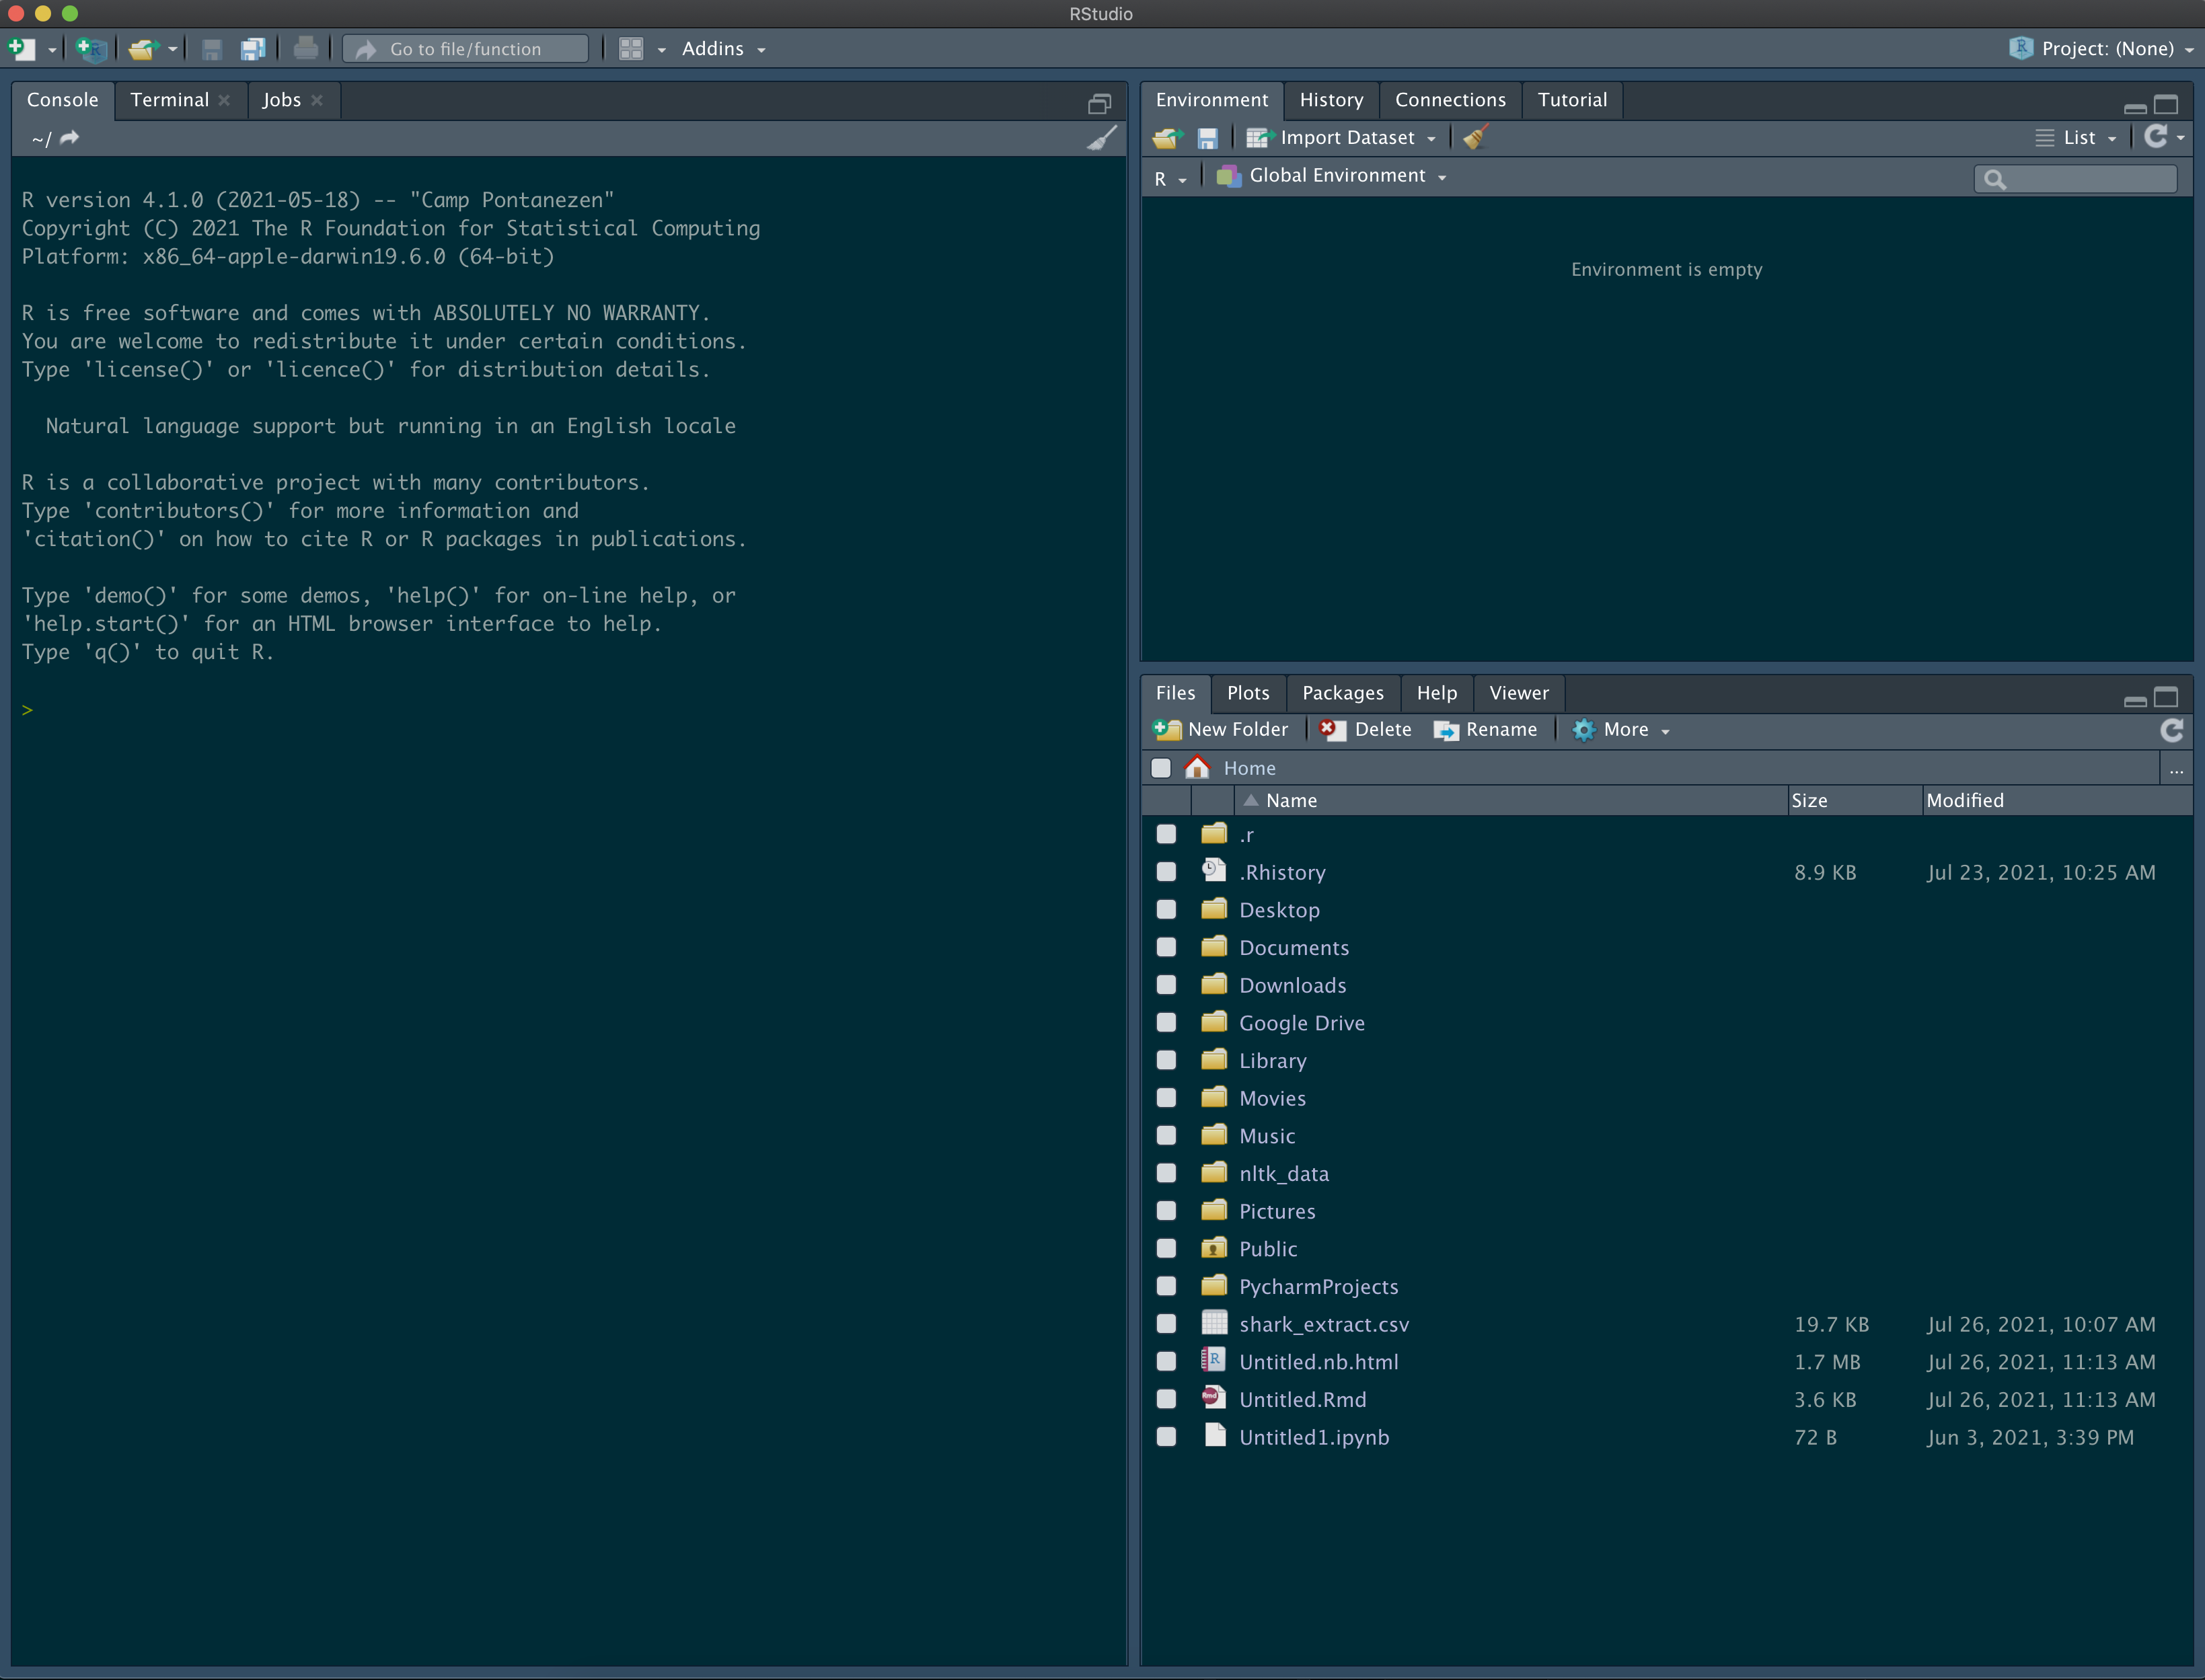
\includegraphics[width=.5\linewidth]{img1.png}
  \label{fig:boat1}
  \centering
\end{figure}

\miquestion \textbf{Instalar paquetes necesarios}
R es un software que requiere instalar paquetes. El paquete que vamos a requerir para este primer laboratorio es tidyverse:

\begin{itemize}
\item Instalar tidyverse: En la consola poner \textbf{install.packages('tidyverse')}
\item Cargar tidyverse: En la consola poner \textbf{library(tidyverse)}. Este paso debe repetirse cada vez que se inicie R.
\end{itemize}


\miquestion \textbf{Correr el laboratorio}

\begin{itemize}
\item Para correr laboratorio, abre en Rstudio el archivo \textbf{Assignment01.Rmd}. Asegurate de contar con el archivo \textbf{shark\_extract.csv} en la misma ruta.
\item El notebook tiene chunks que puedes ir corriendo uno a uno. Asegurate de correr toda la primer sección
\item Basado en los resultados que te dieron, contesta el  quiz en Canvas
\end{itemize}

\end{questions}

\end{document}